\appendix
\chapter{Glossar}

\paragraph{Guest -} a visitor of the website.
\paragraph{User -} the user type relating to the wiki permissions.
\paragraph{Mod -} the user type relating to the wiki permissions. 
\paragraph{Admin -} the user type relating to the wiki permissions. 
\paragraph{(Wiki) Content -} a page in the wiki. Could belong to News, BSI catalogue, articles or archived versions of all of the above.
\paragraph{Article -} a page in the wiki which was created by a user and does not belong to the News or BSI catalogue.
\paragraph{Threat -} as defined by the BSI Grundschutzkatalog (Gef\"ahrdung).
\paragraph{Measure -} as defined by the BSI Grundschutzkatalog (Ma\ss nahme).

\chapter{Use Case Diagrams}

\begin{figure}[h] 
    \centering
    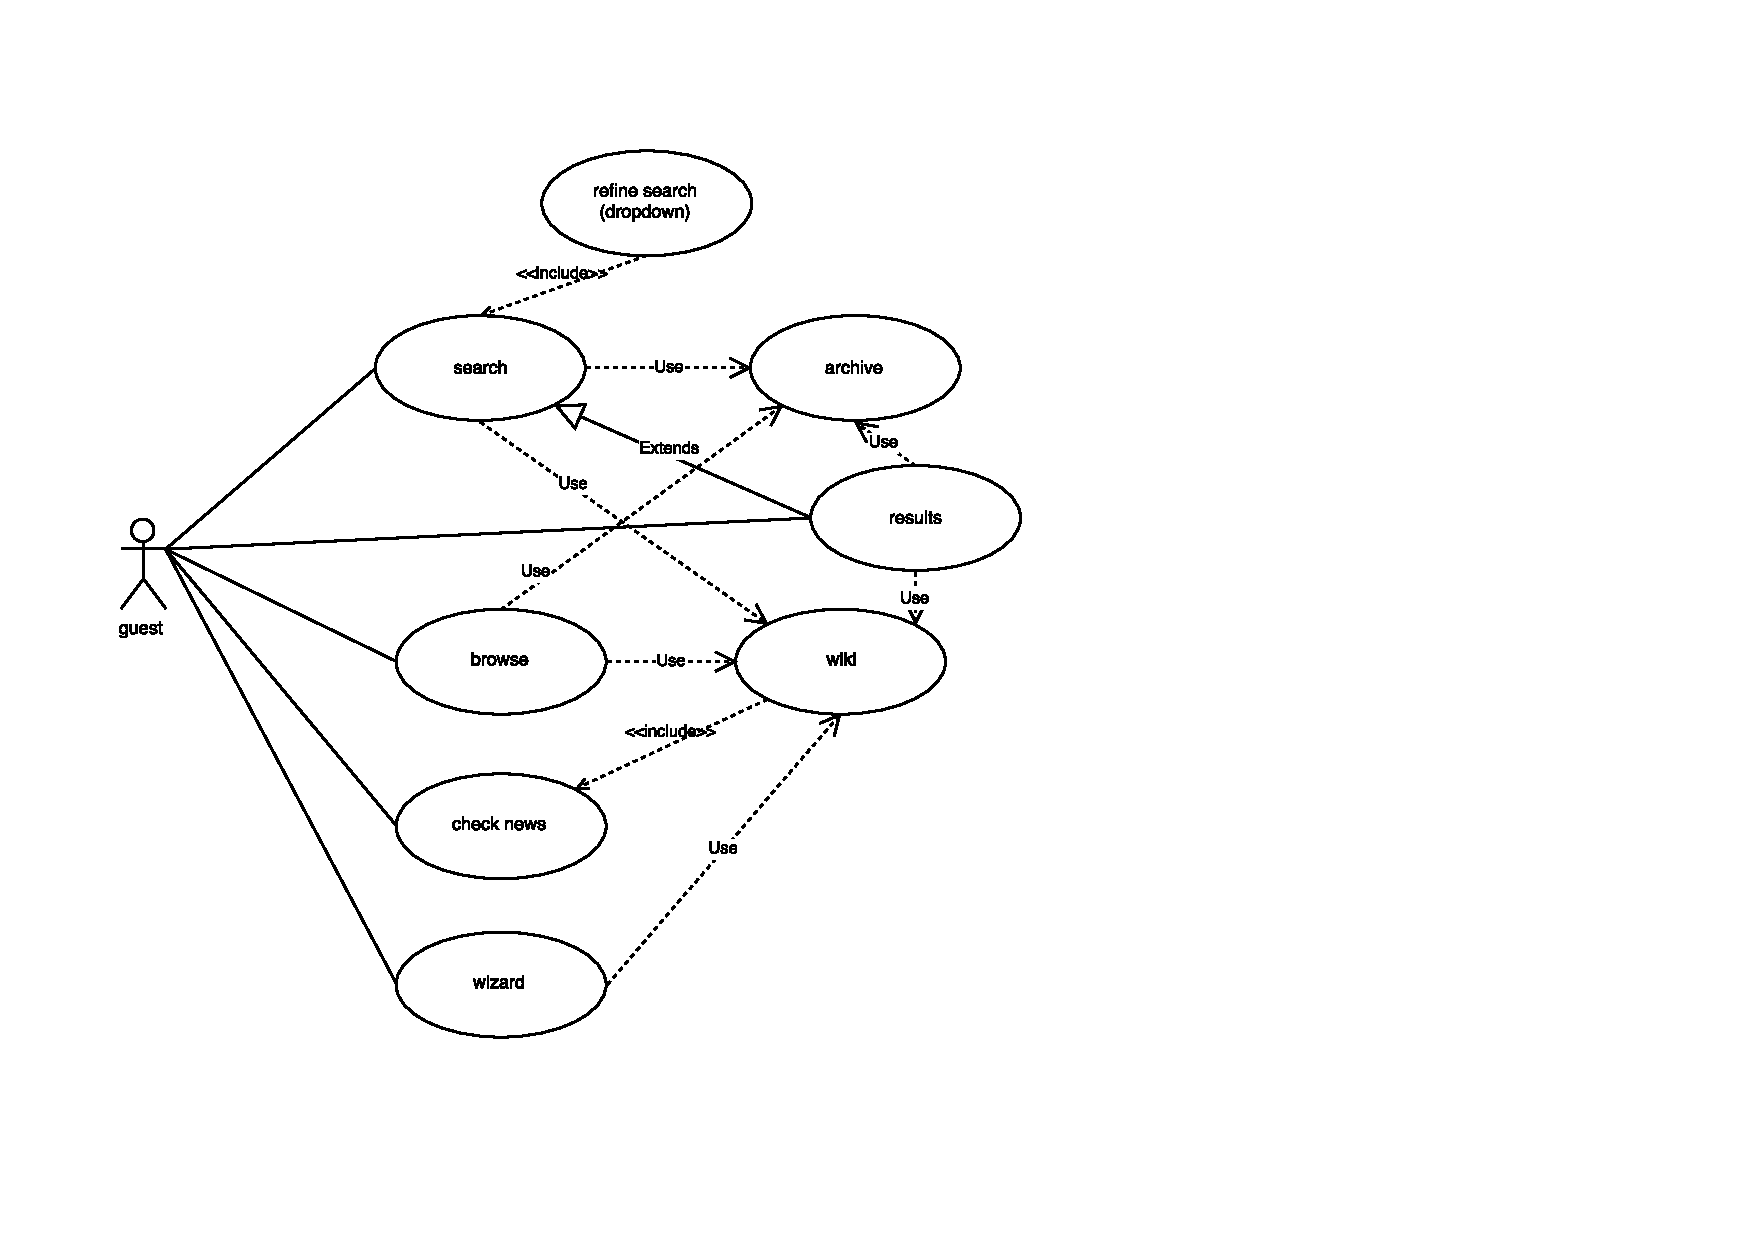
\includegraphics[scale=1.0]{Pictures/Guest}
    \caption{guest - use case}
\end{figure}

\begin{figure}[h] 
    \centering
    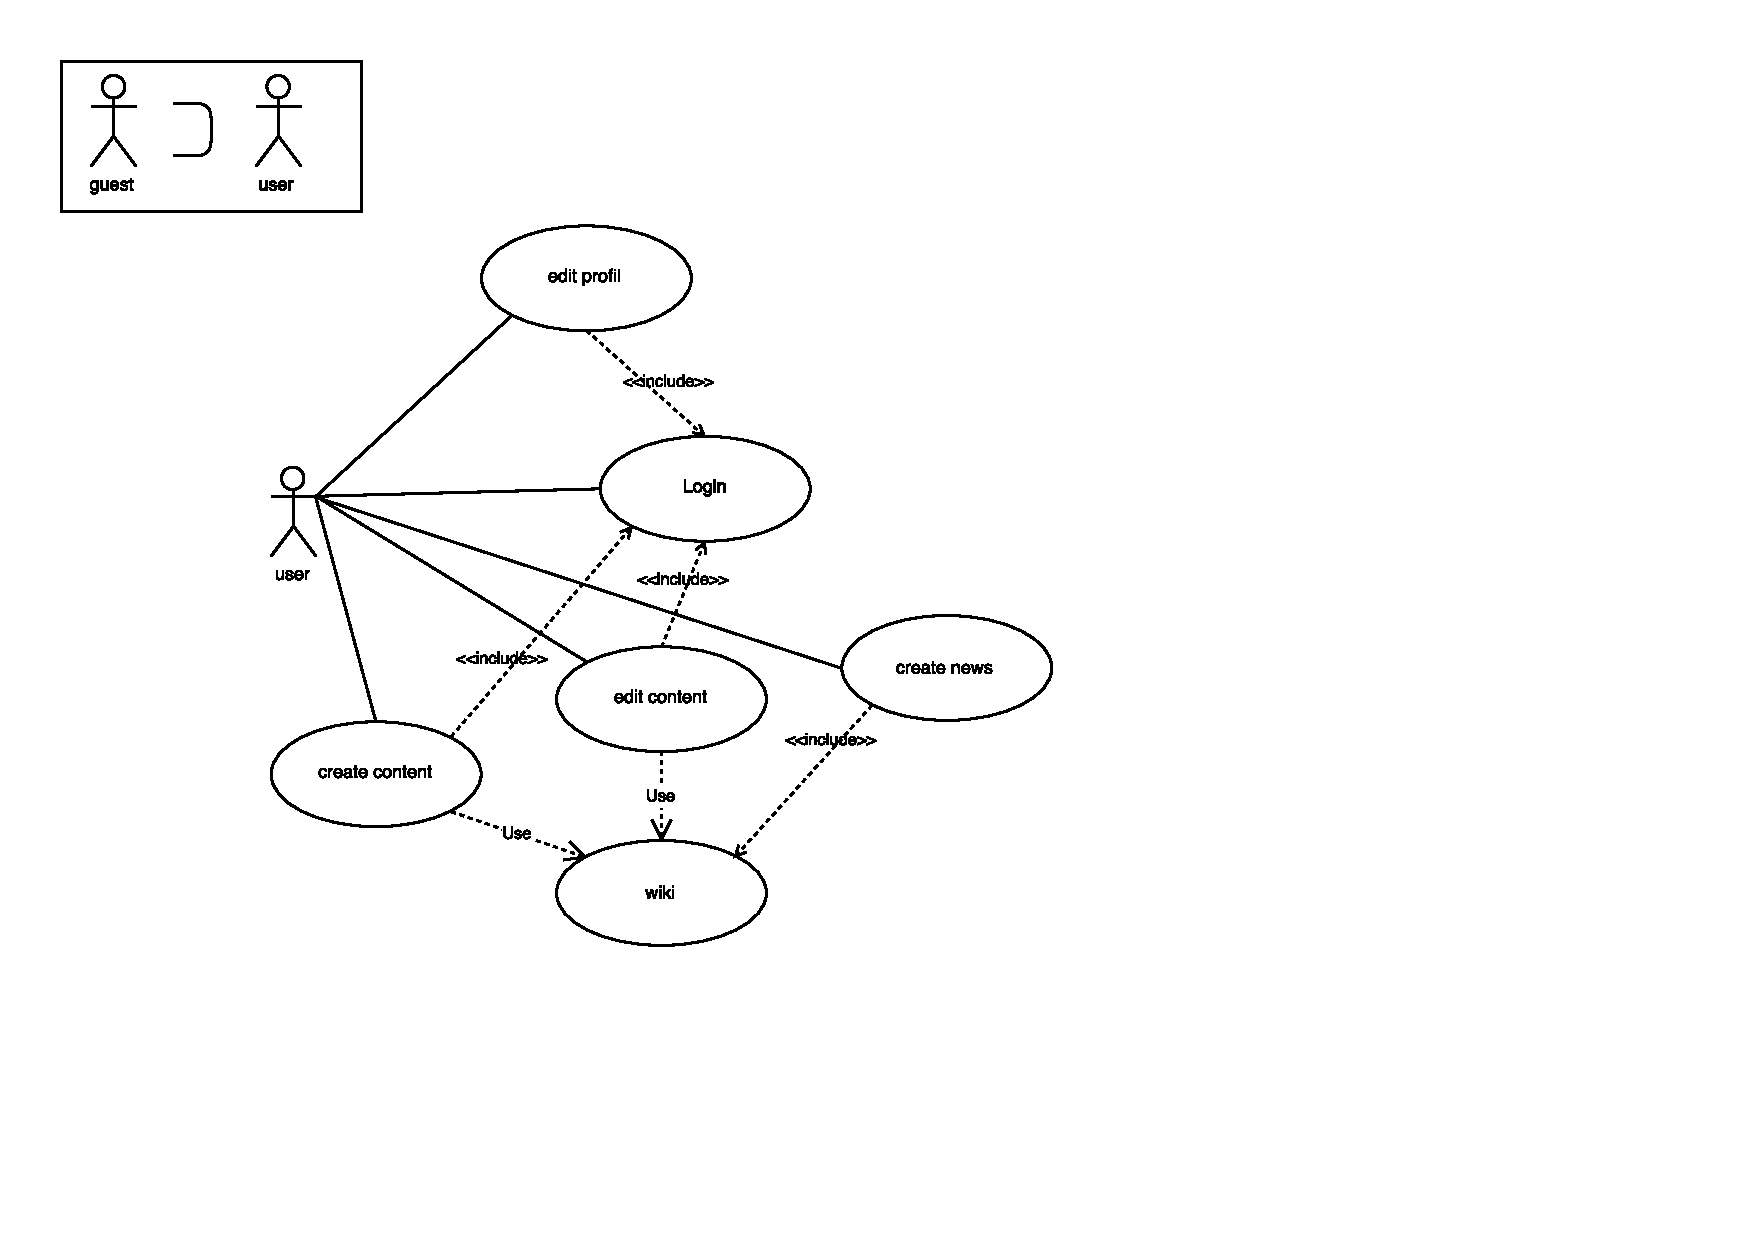
\includegraphics[scale=1.0]{Pictures/User}
    \caption{user - use case}
\end{figure}

\begin{figure}[h] 
    \centering
    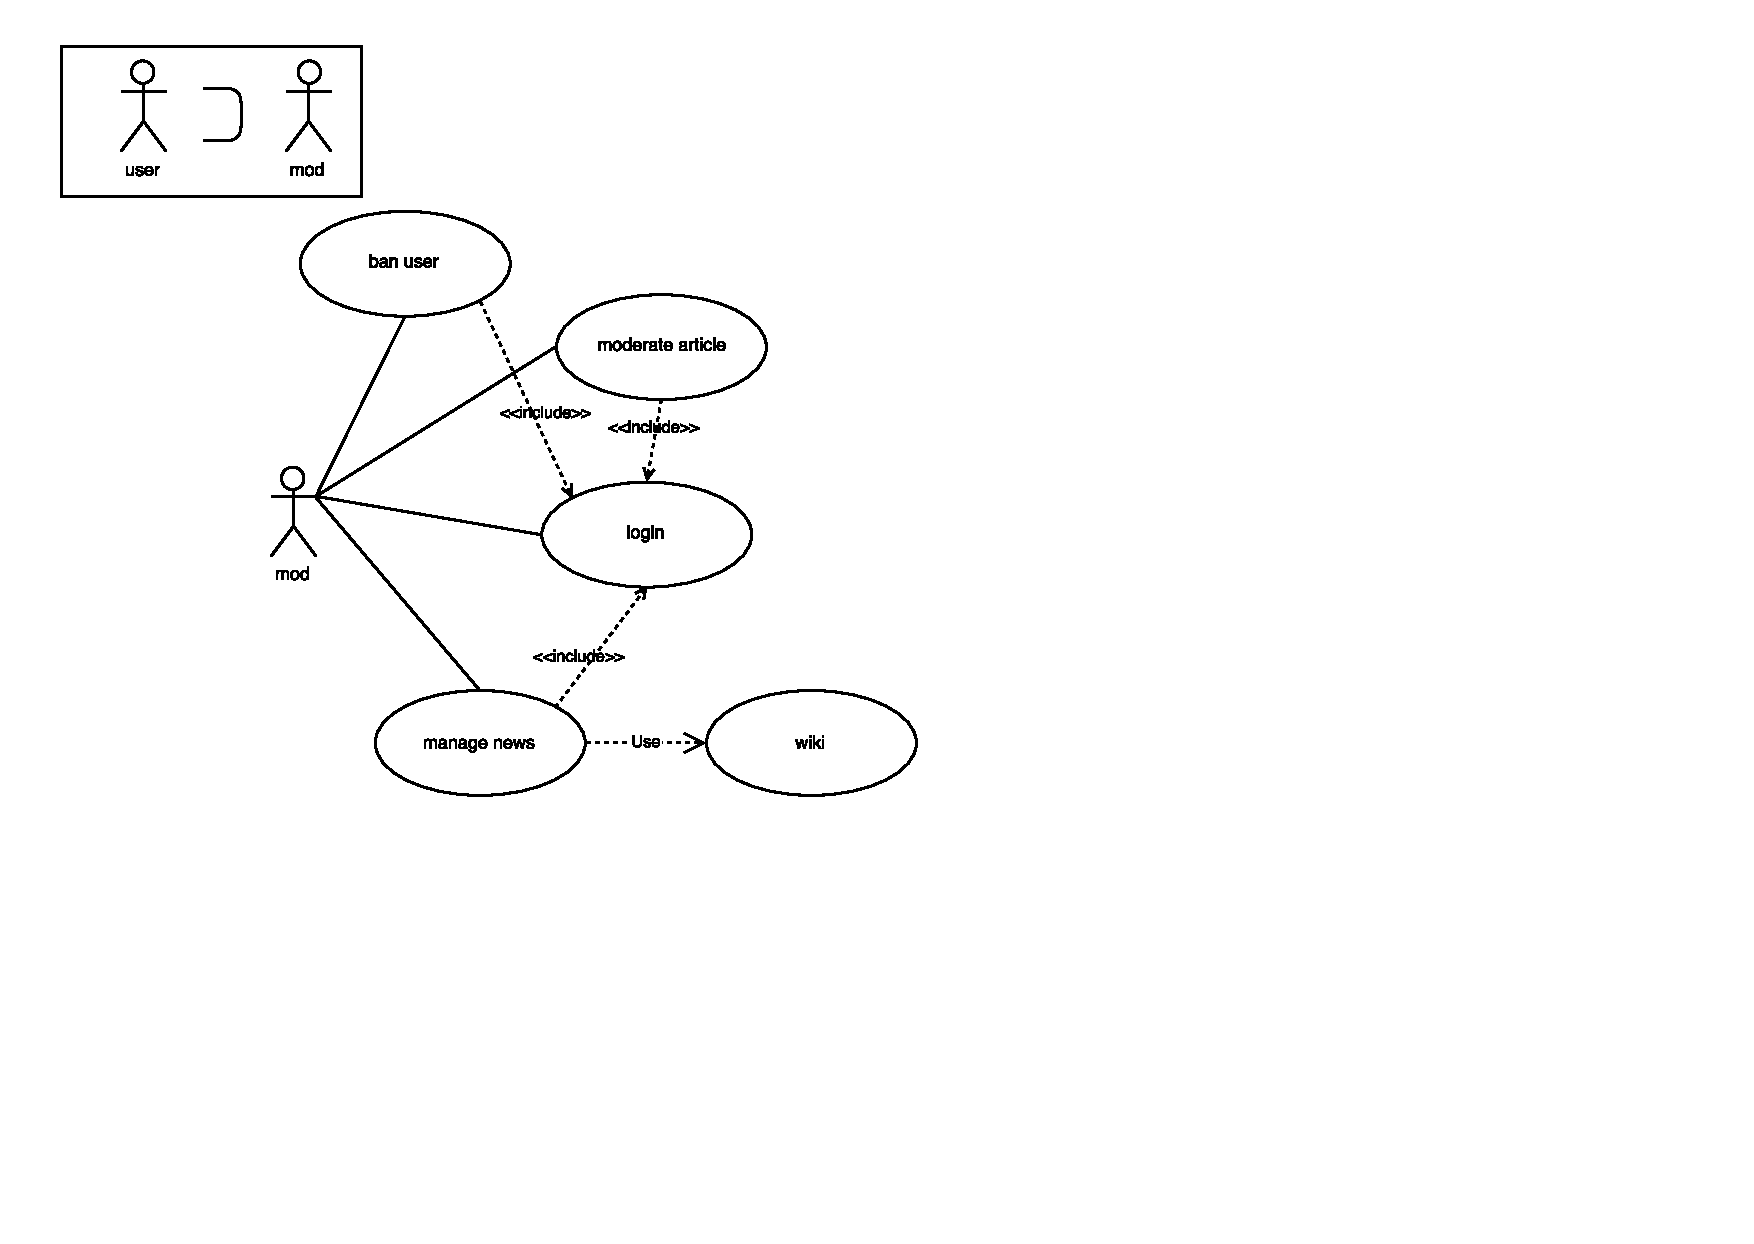
\includegraphics[scale=1.0]{Pictures/Mod}
    \caption{mod - use case}
\end{figure}

\begin{figure}[h]  
    \centering
    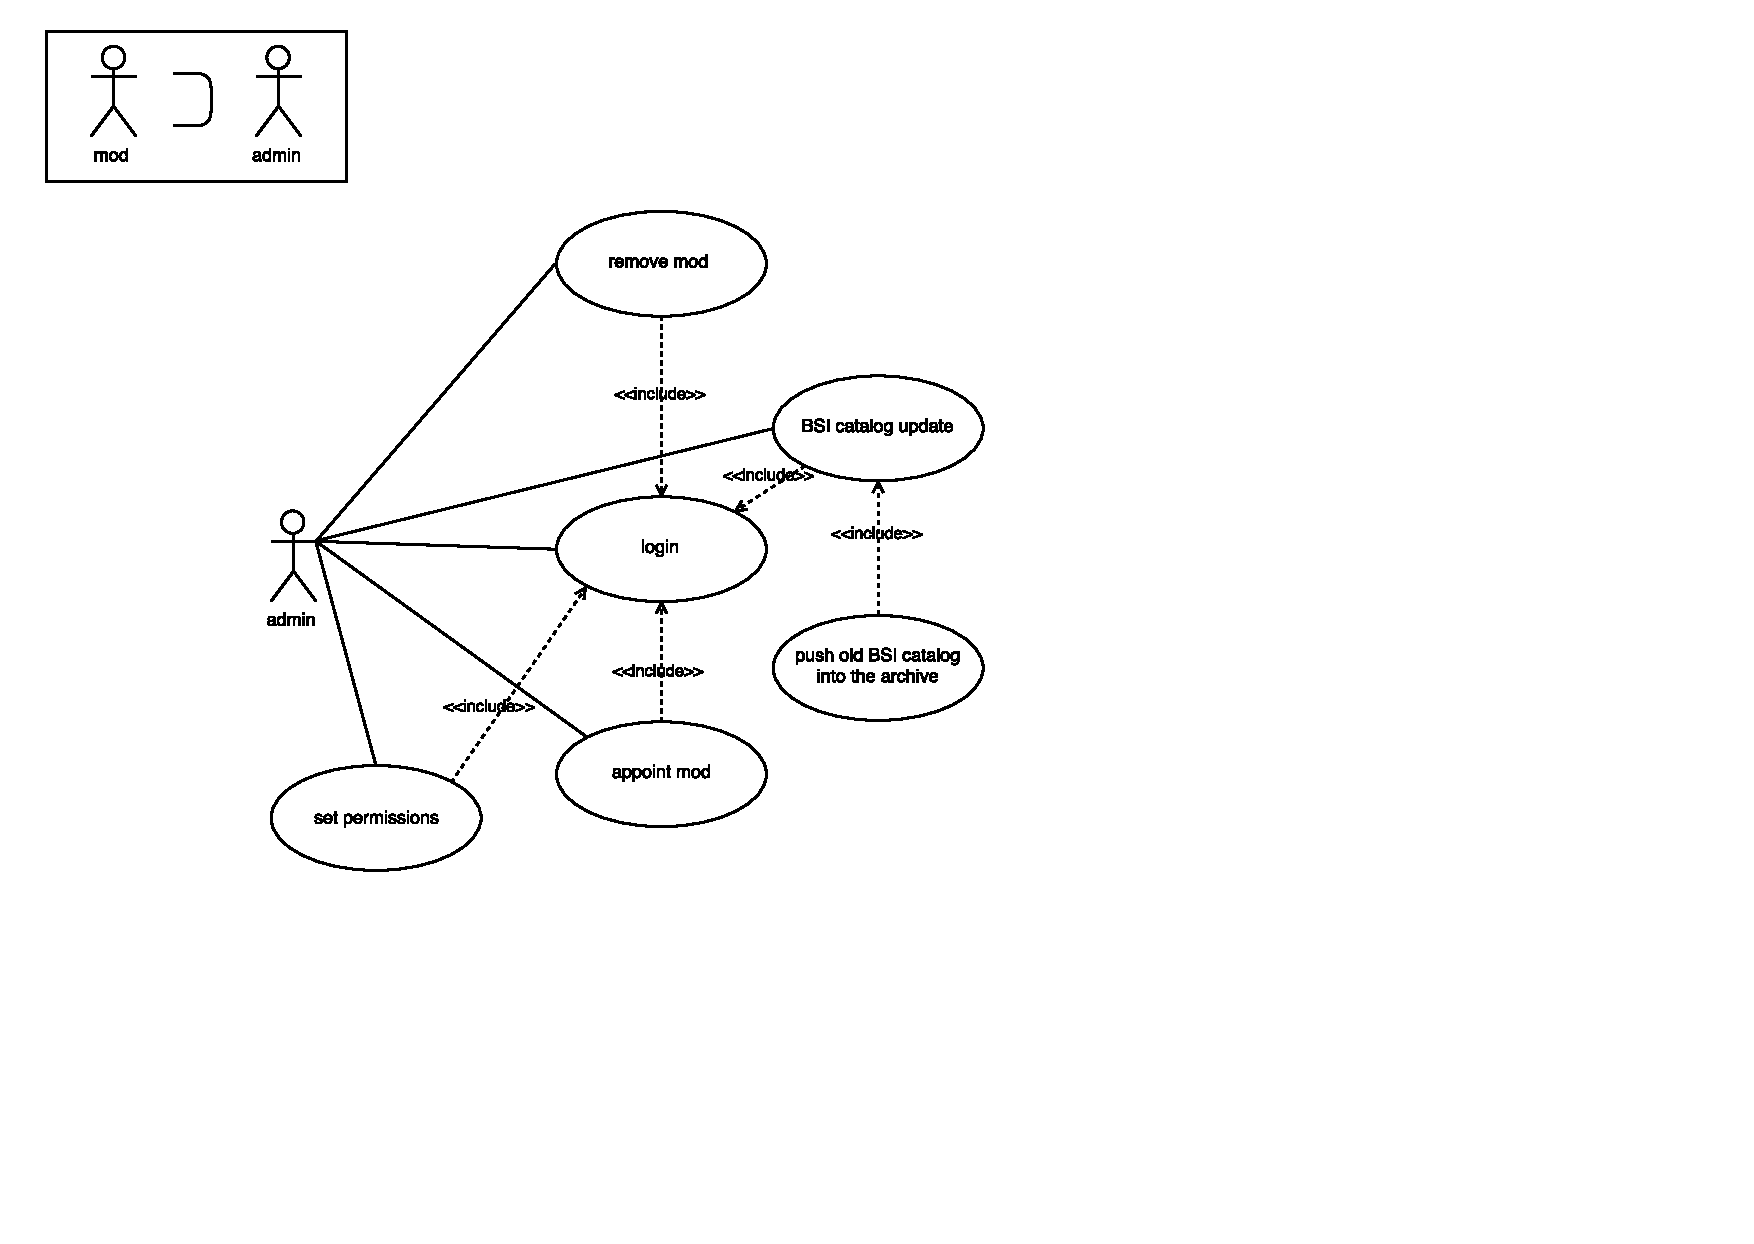
\includegraphics[scale=1.0]{Pictures/Admin}
    \caption{admin - use case}
\end{figure}
 

\chapter{BSI Pages}

\section{Structure of BSI Pages}
\label{appendix_bsi}

\begin{figure}[h]  
    \centering
    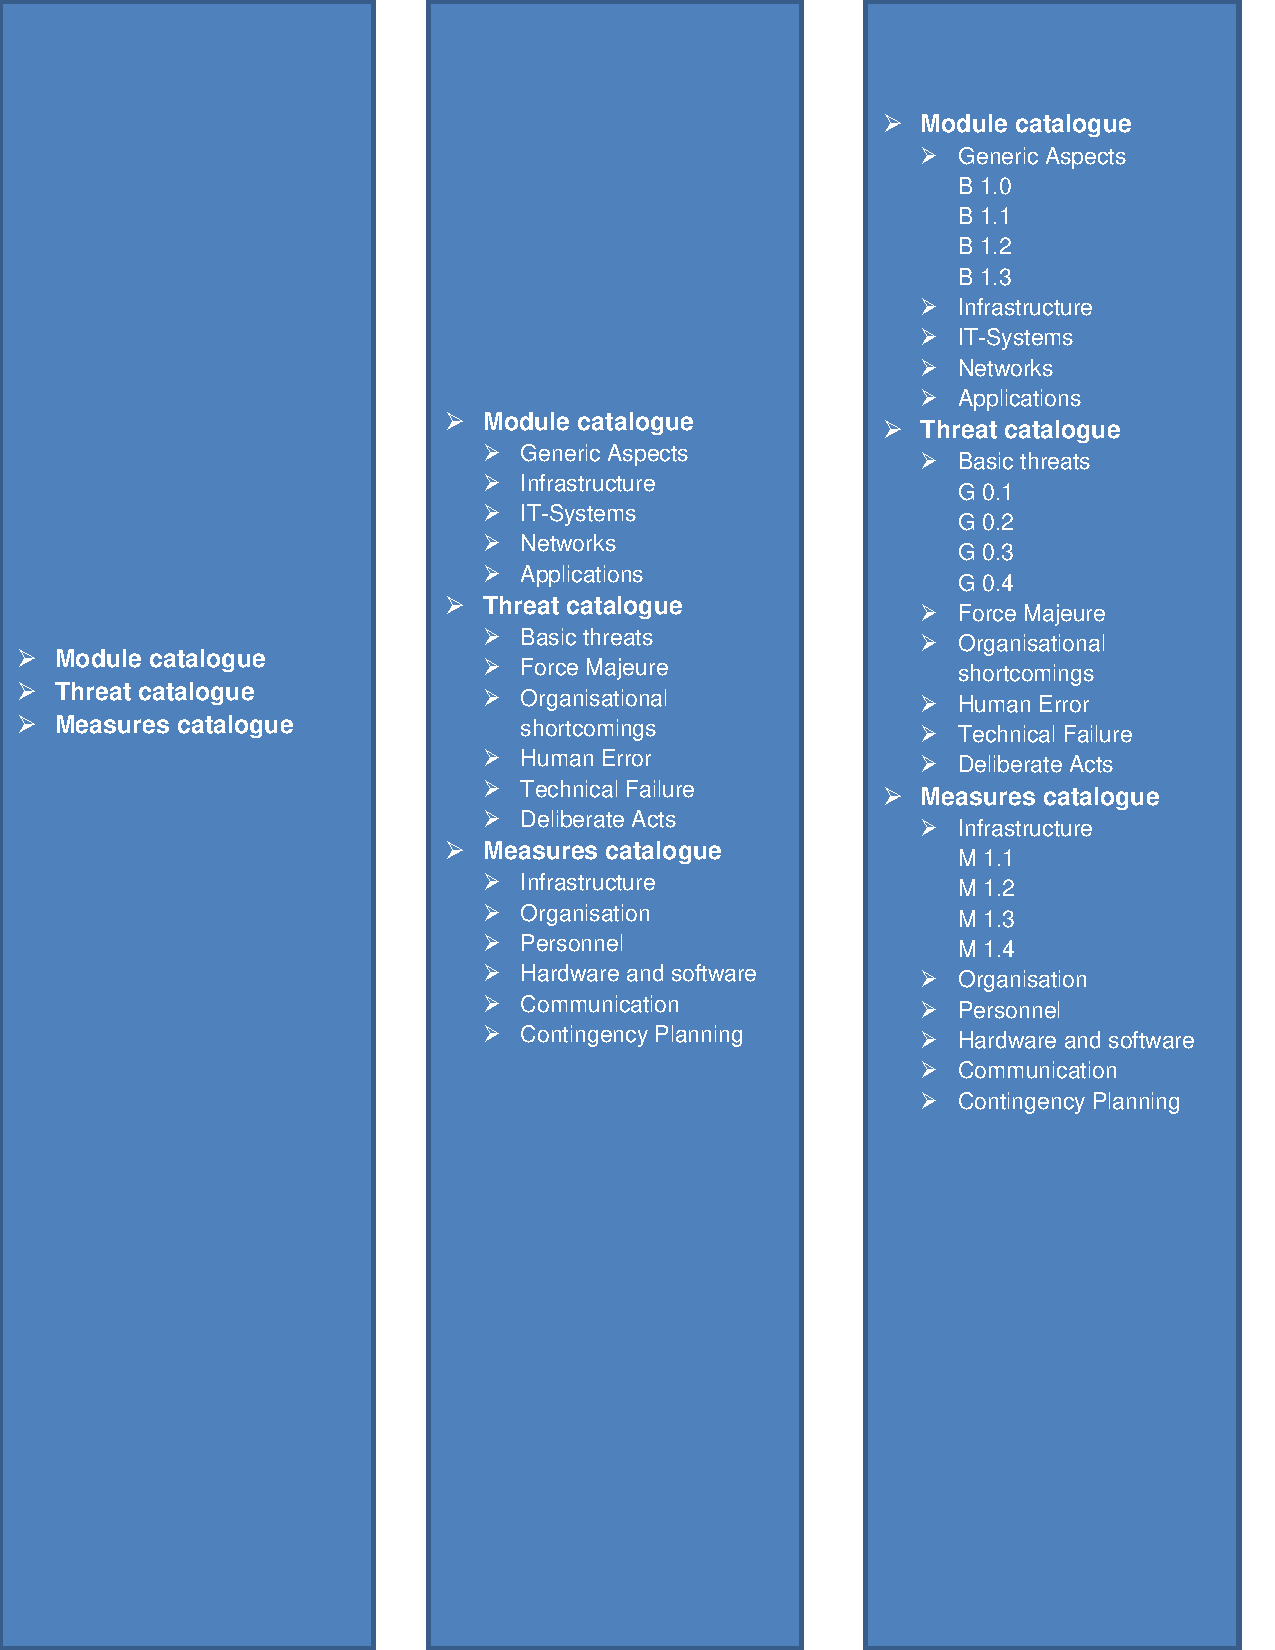
\includegraphics[page=1,width=.8\textwidth]{Pictures/bsi_pages.pdf}
    \caption{Tree view of BSI pages.}
\end{figure}

\begin{figure}[h]  
    \centering
    \includegraphics[page=2,width=.8\textwidth]{Pictures/bsi_pages.pdf}
    \caption{BSI page showing a building block page sorted by threats.}
\end{figure}

\begin{figure}[h]  
    \centering
    \includegraphics[page=4,width=.8\textwidth]{Pictures/bsi_pages.pdf}
    \caption{BSI page showing a building block page sorted by measures.}
\end{figure}

\section{Linking to BSI Pages}
\label{appendix_bsi_link}

\begin{figure}[h]  
    \centering
    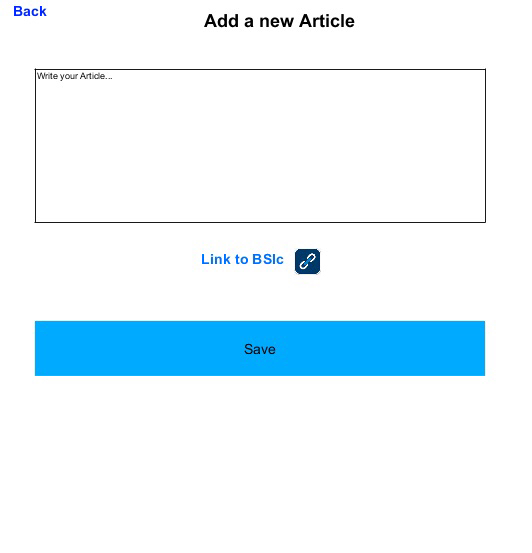
\includegraphics[page=1,width=.8\textwidth]{Pictures/link_to_bsi_1.jpg}
    \caption{The editing page to write an article features the option for users to link their article.}
\end{figure}

\begin{figure}[h]  
    \centering
    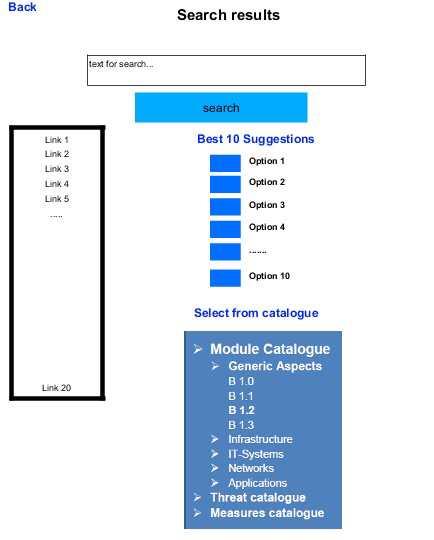
\includegraphics[page=1,width=.8\textwidth]{Pictures/link_to_bsi_2.jpg}
    \caption{When users want to link their articles they can search for keywords or browse the catalogue.They always see their already linked pages. }
\end{figure}



\begin{figure}[h]  
    \centering
    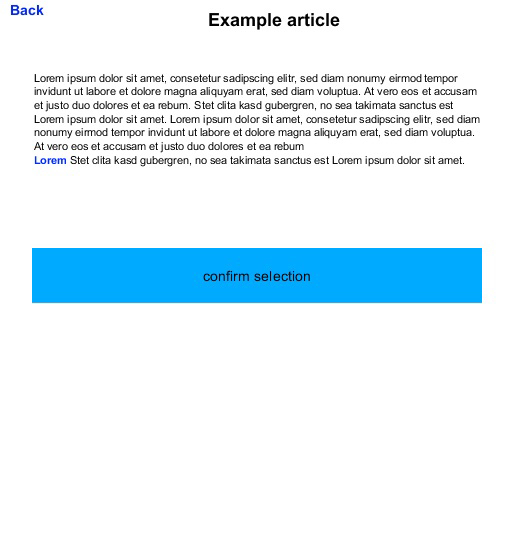
\includegraphics[page=1,width=.8\textwidth]{Pictures/link_to_bsi_3.jpg}
    \caption{Users select a word on a BSI page and confirm their selection.}
\end{figure}

